% `advanced_example.tex', an advanced example employing the AIAA class
% plus other third-party LaTeX packages.
%
% For a bare-bones usage, see `template.tex'.
%
% Typical processing for PostScript (PS) output:
%
%  latex advanced_example
%  bibtex advanced_example  (bibliography)
%  makeindex -s nomencl.ist -o advanced_example.gls advanced_example.glo
%                            (nomenclature)
%  latex advanced_example   (repeat as needed to resolve references)
%
%  xdvi advanced_example    (onscreen draft display)
%  dvips advanced_example   (postscript)
%  gv advanced_example.ps   (onscreen display)
%  lpr advanced_example.ps  (hardcopy)
%
% With the above, only Encapsulated PostScript (EPS) images can be used.
%
%
%  pdflatex advanced_example
%  bibtex advanced_example    (bibliography)
%  makeindex -s nomencl.ist -o advanced_example.gls advanced_example.glo
%                              (nomenclature)
%  pdflatex advanced_example  (repeat as needed to resolve references)
%
%  acroread advanced_example.pdf  (onscreen display)
%
% If you have EPS figures, you will need to use the epstopdf script
% to convert them to PDF because PDF is a limmited subset of EPS.
% pdflatex accepts a variety of other image formats such as JPG, TIFF,
% PNG, and so forth -- check the documentation for your version.
%
% If you do *not* specify suffixes when using the graphicx package's
% \includegraphics command, latex and pdflatex will automatically select
% the appropriate figure format from those available.  This allows you
% to produce PS and PDF output from the same LaTeX source file.
%
% To generate a large format (e.g., 11"x17") PostScript copy for editing
% purposes, use
%
%  dvips -x 1467 -O -0.65in,0.85in -t tabloid advanced_example
%
% For further details and support, read the Users Manual, aiaa.pdf.

\documentclass[]{aiaa-tc}% insert '[draft]' option to show overfull boxes

 \usepackage{varioref}%  smart page, figure, table, and equation referencing
 \usepackage{wrapfig}%   wrap figures/tables in text (i.e., Di Vinci style)
 \usepackage{threeparttable}% tables with footnotes
 \usepackage{dcolumn}%   decimal-aligned tabular math columns
  \newcolumntype{d}{D{.}{.}{-1}}
 \usepackage{nomencl}%   nomenclature generation via makeindex
  \makeglossary
 \usepackage{amssymb,amsmath}
 \usepackage{subfigure}% subcaptions for subfigures
 \usepackage{subfigmat}% matrices of similar subfigures, aka small mulitples
 \usepackage{fancyvrb}%  extended verbatim environments
 \fvset{fontsize=\footnotesize,xleftmargin=2em}
 \usepackage{lettrine}%  dropped capital letter at beginning of paragraph
%  \usepackage[dvips]{dropping}% alternative dropped capital package
 \usepackage[colorlinks]{hyperref}%  hyperlinks [must be loaded after dropping]
 \usepackage{float}
 \usepackage{longtable,booktabs,tabularx}
 % \restylefloat{table}
 \usepackage{graphicx}
 \usepackage{caption}
 \usepackage{siunitx}
 \usepackage{multicol}
 \usepackage{indentfirst}
 \usepackage{environ}
 \usepackage[labelfont=bf]{caption}
 \usepackage{multirow}
 \usepackage{setspace}
%  \graphicspath{{./figs/}}
 \usepackage[sort, numbers]{natbib}

\usepackage{bm}
%\title{Conceptual Design of an Extremely Short Takeoff and Landing Aircraft (using GPkit/for Urban Air Mobility)}
\title{Feasibility Study of Short Takeoff and Landing Urban Air Mobility Vehicles using Geometric Programming}
 \author{
  Chris Courtin\thanks{Graduate Student, Aeronautics and Astronautics Engineering, MIT, 77 Mass Ave, Cambridge MA, 02139, AIAA Member.}, 
  Michael Burton\thanks{Graduate Student, Aeronautics and Astronautics Engineering, MIT, 77 Mass Ave, Cambridge MA, 02139, AIAA Student.}, 
  Patrick Butler\thanks{Graduate Student, Aeronautics and Astronautics Engineering, MIT, 77 Mass Ave, Cambridge MA, 02139, AIAA Student.}, 
  Alison Yu\thanks{Graduate Student, Aeronautics and Astronautics Engineering, MIT, 77 Mass Ave, Cambridge MA, 02139, AIAA Student.}, 
 Parker Vascik \thanks{Graduate Student, Aeronautics and Astronautics Engineering, MIT, 77 Mass Ave, Cambridge MA, 02139, AIAA Student.}, 
  John Hansman\thanks{T. Wilson Professor, Aeronautics and Astronautics Engineering, MIT, 77 Mass Ave, Cambridge MA, 02139, AIAA Member.} \\
  {\normalsize\itshape
   Massachusetts Institute of Technology, Cambridge, 02139, USA}\\
 }

 % Data used by 'handcarry' option
 \AIAApapernumber{YEAR-NUMBER}
 \AIAAconference{Conference Name, Date, and Location}
 \AIAAcopyright{\AIAAcopyrightD{YEAR}}

 % Define commands to assure consistent treatment throughout document
 \newcommand{\eqnref}[1]{(\ref{#1})}
 \newcommand{\class}[1]{\texttt{#1}}
 \newcommand{\package}[1]{\texttt{#1}}
 \newcommand{\file}[1]{\texttt{#1}}
 \newcommand{\BibTeX}{\textsc{Bib}\TeX}
 \usepackage{hyperref}
 \hypersetup{citecolor = blue}

\begin{document}

\graphicspath{{./figs/}}
\maketitle

\begin{abstract}
    The feasibility of an Urban Air Mobility (UAM) system that features electric Extremely Short Takeoff and Landing (ESTOL) vehicles is investigated.  An overview is given of the system constraints that must be incorporated into the design of the vehicle.  The system-wide advantages and limitations of ESTOL aircraft are discussed, for both near- and far-term system implementations.  A detailed vehicle sizing model is developed using geometric programming, a robust optimization framework.  This model is used to determine feasible boundaries on required runway size, vehicle range, and the sensitivity of the vehicle design to high-level mission parameters such as speed and number of passengers.  Key unique drivers of the vehicle design are identified.  The impact of distributed electric propulsion (DEP) is assessed.  Performance relative to a comparable Vertical Takeoff and Landing (VTOL) vehicle is analyzed, both with currently available technology and forecasted future technology.   The infrastructure requirements (runway size, approach paths, etc.) needed to support ESTOL operations are assessed according to current regulations.  Two major urban areas (Boston and Los Angeles) are presented as case studies to show where this infrastructure could be feasibly located.  Key challenges and risks to implementation are discussed.  


\end{abstract}

\section*{Nomenclature}

\begin{multicols}{2}
\small

\begin{tabbing}
  XXXXXXX \= \kill% this line sets tab stop
$A$ \> takeoff helper variable \\
$AR$ \> wing aspect ratio \\
$b$ \> wing span \\ % [ft] \\
$B$ \> takeoff helper variable \\
$c$ \> wing chord \\ %[m] \\
$C_D$ \> drag coefficient \\
$CDA$ \> area drag coefficient \\
$C_{D_g}$ \> ground drag coefficient \\
$c_{d_p}$ \> wing profile drag coefficient \\
$C_L$ \> lift coefficient \\
$C_{L_g}$ \> ground lift coefficient \\
$C_{L_{\mathrm{max}}}$ \> max lift coefficient \\
$D$ \> drag \\
$e$ \> span efficiency \\
$f_{\mathrm{struct}}$ \> fractional structural weight \\
$g$ \> gravitational constant \\
$L$ \> lift \\
$\mathcal{M}_{\mathrm{root}}$ \> root moment stress \\
$N$ \> deceleration factor \\
$P_{\mathrm{shaft-max}}$ \> max shaft power \\
$P_{\mathrm{spec}}$ \> specific motor power \\
$Re$ \> Reynolds number \\
$S$ \> wing area \\
$S_{\mathrm{land}}$ \> landing ground roll \\
$S_{\mathrm{runway}}$ \> runway distance \\
$S_{\mathrm{TO}}$ \> take off ground roll \\
$S_{y_{\mathrm{spar}}}$ \> spar section modulus \\
$t$ \> time \\
$T$ \> thrust \\
$V$ \> speed \\
$V_{\mathrm{stall}}$ \> stall speed \\
$W_{\mathrm{batt}}$ \> battery weight \\
$W_{\mathrm{fadd}}$ \> additional wing weight\\
$W_{\mathrm{motor}}$ \> motor weight \\
$W_{\mathrm{MTO}}$ \> max take off weight \\
$W_{\mathrm{pay}}$ \> payload weight \\
$W_{\mathrm{skin}}$ \> wing skin weight \\
$W_{\mathrm{spar}}$ \> wing spar weight \\
$W_{\mathrm{struct}}$ \> structural weight \\
$W_{\mathrm{wing}}$ \> wing weight \\
$\eta_{\mathrm{elec}}$ \> combined electric efficiency \\
$\eta_{\mathrm{prop}}$ \> propeller efficiency \\
$\mu$ \> rolling friction coefficient \\
$\rho$ \> air density \\
$\sigma_{\mathrm{CFRP}}$ \> carbon fiber allowable stress \\
 \end{tabbing}

\end{multicols}
% \printglossary% creates nomenclature section produced by MakeIndex

\section{Introduction}
Urban Air Mobility (UAM) is a broad concept that refers to a set of related operations and technologies that aim to provide on-demand intra-city and regional air transportation.  UAM concepts of some form or another have been around for at least the past fifty years.  Helicopters have been performing UAM-type missions since the 1960’s and have sufficient performance capability to meet nearly all payload, speed, and range requirements of the current UAM mission profile. However, historical helicopter public transportation networks by and large did not succeed and do not exist today due to the high costs of helicopter operation, the high noise generation of these vehicles, and the poor safety record of these aircraft.  Recently, advances in electric vehicle propulsion and key subsystem technologies has opened up the vehicle design space and enabled new approaches to mitigating some of these systemic challenges.  This has sparked renewed interest in the UAM concept and the development of UAM-specific vehicles.  Numerous legacy and emerging aircraft manufacturers are developing vehicles for this mission with novel configurations that leverage more-electric or all-electric vehicles and propulsion systems.  

There are a variety of system architectures that are being considered for UAM vehicles. Figure~\ref{f:ov} shows some of the most popular options, organized by number of propulsors and method of lift generation.  Of these architecture options, powered-lift distributed electric propulsion (DEP) and rotor-lift DEP are currently the two being most actively pursued. Powered-lift DEP is seen as being especially promising due to its VTOL capability and relatively efficient, high-speed cruise compared to a pure rotorcraft.  These vehicle concepts may have noise benefits compared to conventional helicopters.  These benefits arise in part from the lack of engine noise as well as the design freedom to vary tip speed and disk loading, both of which are key noise drivers. 
\begin{figure}
\begin{center}
	
\includegraphics[width=.75\textwidth]{vehicle_architectures.png}
\caption{Overview of potential UAM aircraft system architectures}
\label{f:ov}
\end{center}
\end{figure}

However, there are still significant challenges associated with these vehicle architectures.  First, the certification pathway for all-electric, fly-by-wire aircraft are not defined and represent a significant potential delay for system implementation in the United States. Secondly, it is unclear that noise can be reduced sufficiently with these configurations to the level that will allow widespread community acceptance.  Finally, the VTOL mission segment, reliance on lithium-ion batteries, and fly-by-wire features of these aircraft present significant safety issues that may be complex and costly to mitigate. 

One vehicle architecture which has not been widely considered for the UAM mission is the extremely short takeoff and land (ESTOL) aircraft, which is a fixed-wing aircraft capable of operating off a runway of 100-500ft.  By utilizing the wing throughout all phases of flight, ESTOL aircraft have performance advantages compared to VTOL aircraft of similar payload capacity.  If the runway can be made sufficiently short, the infrastructure differences between VTOL and ESTOL become relatively insignificant, and a useful network of runways can be constructed in close proximity to a major urban area.  ESTOL also has advantages over VTOL in noise and vehicle certification, which are two of the highest barriers to implementation of a function UAM system.  However, it is unclear how short a runway a vehicle could realistically be made to operate from, and how that requirement trades with speed, range, and payload.  

This research paper conducts an in-depth analysis of the feasibility of an UAM system that features ESTOL aircraft, considering both infrastructure and vehicle design constraints.  To conduct the vehicle design trade studies, a geometric programming (GP) vehicle sizing and performance model is developed to rapidly and holistically consider the large design space.  Ground infrastructure and approach path constraints are internalized in this model as design constraints on the aircraft.  This model is exercised to determine feasible bounds on runway operating length, and how vehicle range, speed, and payload capacity trade with ground infrastructure requirements.  
To assess the ground infrastructure requirements, the current FAA guidance for airport design and approach path layouts is used to create the nominal layout for a short takeoff and landing area (STOLA).  The feasibility of locating these STOLA near major urban areas is assessed by looking at case studies of two particular cities, Boston and Los Angeles.  The potential for ESTOL aircraft to act as a pathway to the development of large-scale UAM systems is reviewed from a technical, operational and business feasibility perspective. Furthermore, the complementary nature of ESTOL aircraft operations and potential future VTOL UAM operations are hypothesized. As part of this work, previous literature concerning small aircraft transportation system design ~\cite{Viken}, ~\cite{Holmes}, thin-haul transportation vehicles ~\cite{Harish},~\cite{Kreimeier},~\cite{Justin} �, VTOL aircraft ~\cite{Duffy}, and STOL aircraft is considered ~\cite{Antcliff},~\cite{SeeleyIV}. 

\section{Background}

\paragraph{Current Technology} ESTOL aircraft are not a new concept.  The Helio Courier, first built in the late 1940s, is one existing example, with demonstrated takeoff and landing distances from 100-300ft.  Highly experienced bush pilots are able to achieve landing distances on the order of single aircraft lengths.  Developing an aircraft that can operate of extremely short runways is clearly technologically feasible.  Nevertheless, ESTOL aircraft technology has not found wide adoption outside of the relatively small community of pilots who routinely fly to remote, relatively unimproved landing areas.   There are inherent challenges in taking existing ESTOL aircraft and using them for operations near major urban areas, which are a result of the design penalties that ESTOL capability drove on the vehicles.  
For example, current ESTOL vehicles achieve their short field performance through a combination of low wing loading, high power-to-weight, and extensive use of high-lift systems.  The low wing loading means that both maximum and best cruise speeds are fairly low.  Additionally, it makes the vehicles highly sensitive to gusts and turbulence, an important consideration for passenger operations.   The high-lift systems required are also complex (except with very low wing loadings), which adds a weight and cost penalty to these vehicles.  Depending on the type of powerplant type used, the need for high power at takeoff may also reduce the efficiency at the nominal cruising point.  More significantly, these high-power engines generated substantial noise on takeoff; a primary consideration when operating near urban areas. 

\paragraph{Key Enabling Technologies} The introduction of new electric aircraft technologies has the potential to change the paradigm of current ESTOL aircraft and make them practical for use in an UAM setting.   In the case of an all-electric aircraft, the reduction in noise through the use of batteries and an electric motor is one key area of improvement.  Another is the use of blown lift with distributed electric propulsion, in a configuration similar to the NASA X-57 Maxwell.  This has the ability to generate very high effective lift coefficients (especially on takeoff), with a reduction in the complexity of the high-lift system required and/or an increase in the climb path angle.  This technology allows in increase in the vehicle wing loading, which improves the cruising speed and passenger comfort.  
Additionally, since electric motors can be run above their maximum rated capacity for short periods of time, the weight penalties of installing a high-thrust system that is only needed on takeoff are reduced.  And since most of the motors would be shut down in cruising flight, the propulsion system can be designed to operate at or near peak efficiency throughout most of the mission.  When taken together, these key technologies enable the design of a practical ESTOL vehicle.  The range limitations come mostly from the use of batteries and their poor specific power relative to hydrocarbon fuels; replacing them with a hybrid-electric system could extend the range or reduce vehicle takeoff weight, with associated tradeoffs on noise, emissions, and direct operating cost.  
 
\section{System Design Considerations}

\paragraph{Relationship of ESTOL and VTOL}
The tradeoff between ESTOL/CTOL and VTOL can be simply summarized as a tradeoff between required infrastructure and vehicle performance.  CTOL vehicles generally have higher performance (for most common definition of performance - range, payload capacity, efficiency) than VTOL vehicles, but  require large amounts of ground infrastructure to takeoff and land.  VTOL aircraft pay a significant performance penalty to minimize the amount of ground infrastructure required. ESTOL aircraft lie somewhere in the middle, less infrastructure and performance than CTOL, but more than VTOL.  
When considering a future UAM system, it is unlikely that the entire system will consist of only ESTOL or only VTOL aircraft.  ESTOL, VTOL, and CTOL aircraft all provide different vehicle capabilities and can coexist in a future air transportation network, just as they do today.  For the UAM concept, most of the missions of greatest interest are in the range of 25-100 nmi, with a loading of 1-6 passengers.  These missions will start and/or end in dense urban areas, where CTOL infrastructure cannot be feasibly built.   This mission space can be addressed by either an all-electric ESTOL or VTOL vehicle. ESTOL vehicles have an advantage for longer ranges or higher payloads, while VTOL vehicles have an advantage with highly constrained infrastructure or very short ranges. In a future, fully implemented UAM network that realizes the goal of increased personal mobility and regional connection, there will be a strong demand for both types of capability.  As the underlying technologies mature (batteries, propulsions systems, and vehicle autonomy), both classes of aircraft will increase proportionally in capability, and the capacity of the system as a whole will increase.  The relative advantages of ESTOL and VTOL will likely remain similar.  

\paragraph{The Context of UAM}
It is important to consider the design of an UAM system and vehicle in the context in which it is expected to operate.  Even the most optimistic projections for the development of a UAM system envision it coming about incrementally over the course of the next 10-30 years, primarily paced by improvements in automation technologies, which will effect both direct vehicle control and overall traffic system management.  In this timeframe, there are other transformative transportation technologies on the horizon; semi- and fully- autonomous ground vehicles, Hyperloop systems, and low-cost tunnels to increase road capacity are all technologies being seriously developed that impact the urban mobility market.  It is important to consider how a future air transportation network would interact with and complement all these technologies.  Making most cars autonomous or semi-autonomous may have a much larger impact on surface congestion than replacing a small percentage of car trips with aircraft trips.  For moving large numbers of people short-range point-to-point, tunnels or other high-speed ground infrastructure may be more appropriate than air travel of any kind.  The value proposition of urban air mobility is in how it complements existing and future transportation infrastructure, and enables new connections to be made to high-throughput ground systems.  

\paragraph{Near-term Advantages of ESTOL}
While ESTOL and VTOL aircraft will both be useful in a future UAM network, there are several advantages to developing ESTOL aircraft before VTOL aircraft.  These advantages can be broadly grouped in three categories; regulatory, vehicle, and strategic.  
From a regulatory perspective, ESTOL is advantageous because there is an existing framework for the certification of these types of vehicles.  It is a known configuration, and with the possible exception of the all-electric powertrain can be readily certified under the existing regulatory framework.  Certification of a distributed electric propulsion ESTOL vehicle will advance the technology that underlies VTOL aircraft, and provide a basis for the certification of all future DEP aircraft, within an existing framework.  Additionally, since ESTOL aircraft may not require a fly-by-wire system (at least for initial piloted configurations), the certification process is simpler and more streamlined.  
From a vehicle perspective, the advantages of ESTOL are mostly in performance.  Notably, it allows a higher ratio of pilots to passengers, which could be a critical consideration in early system implementations before vehicle autonomy is fully developed.  It also has advantages in range/payload, noise, and potentially in cost.  \\
However, the main advantages of ESTOL are strategic, in that it minimizes the risks in implementing a new type of air transportation system by focusing on a lower-complexity, more familiar vehicle architecture.  Proof-of-concept vehicles with useful performance characteristics exist.  It advances the underlying UAM technologies within the regulatory and operational environment.  ESTOL vehicles are quieter than VTOL aircraft, especially on approach, which may mitigate one of the primary barriers to adoption of the system.  Additionally, by focusing on slightly longer range regional transit networks, the system may be accessible and useful to a larger percentage of the people living near urban centers who are affected by the negative externalities of the system.  That population may be more accepting of the existing of the system if they can benefit from it.

\section{Infrastructure}
\begin{figure}[!htbp]
\centering
	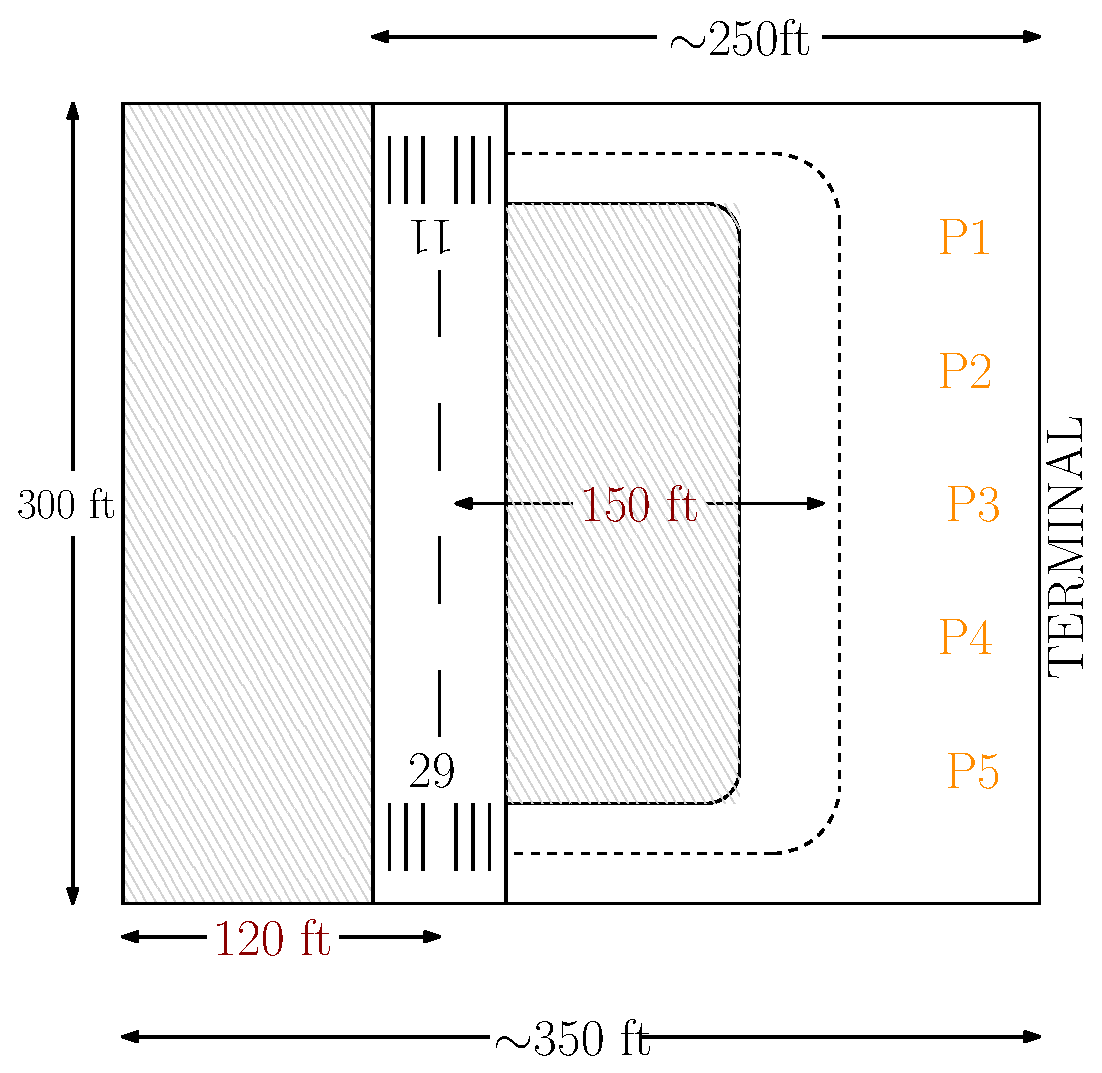
\includegraphics[width=0.5\textwidth]{STOLport_300_nominal.eps}
\caption{The layout of a notional short takeoff and landing area}
\label{fig:stolport}

\end{figure}

Figure ~\ref{fig:stolport} shows the layout of a notional STOLA for a 300ft runway length, taking into account current FAA guidance on runway clearance and centerline separation for runways and taxiways.  This assumes that the vehicles will have an approach reference speed of less than 50 kts.  This layout is notional and is affected by vehicle approach speed and wingspan. 

A key part of the feasibility of an UAM concept is dual-use takeoff and landing areas (TOLA), whether for ESTOL or VTOL vehicles.   Due to the high value and scarcity of undeveloped urban real-estate, single-use UAM infrastructure is likely to be cost-prohibitive.  Considerations for various types of STOLAs are shown in Figure~\ref{fig:stola_key}, which has notional layouts for STOLAs over roads, railways, barges, and buildings. 
\begin{figure}[!htbp]
\centering
	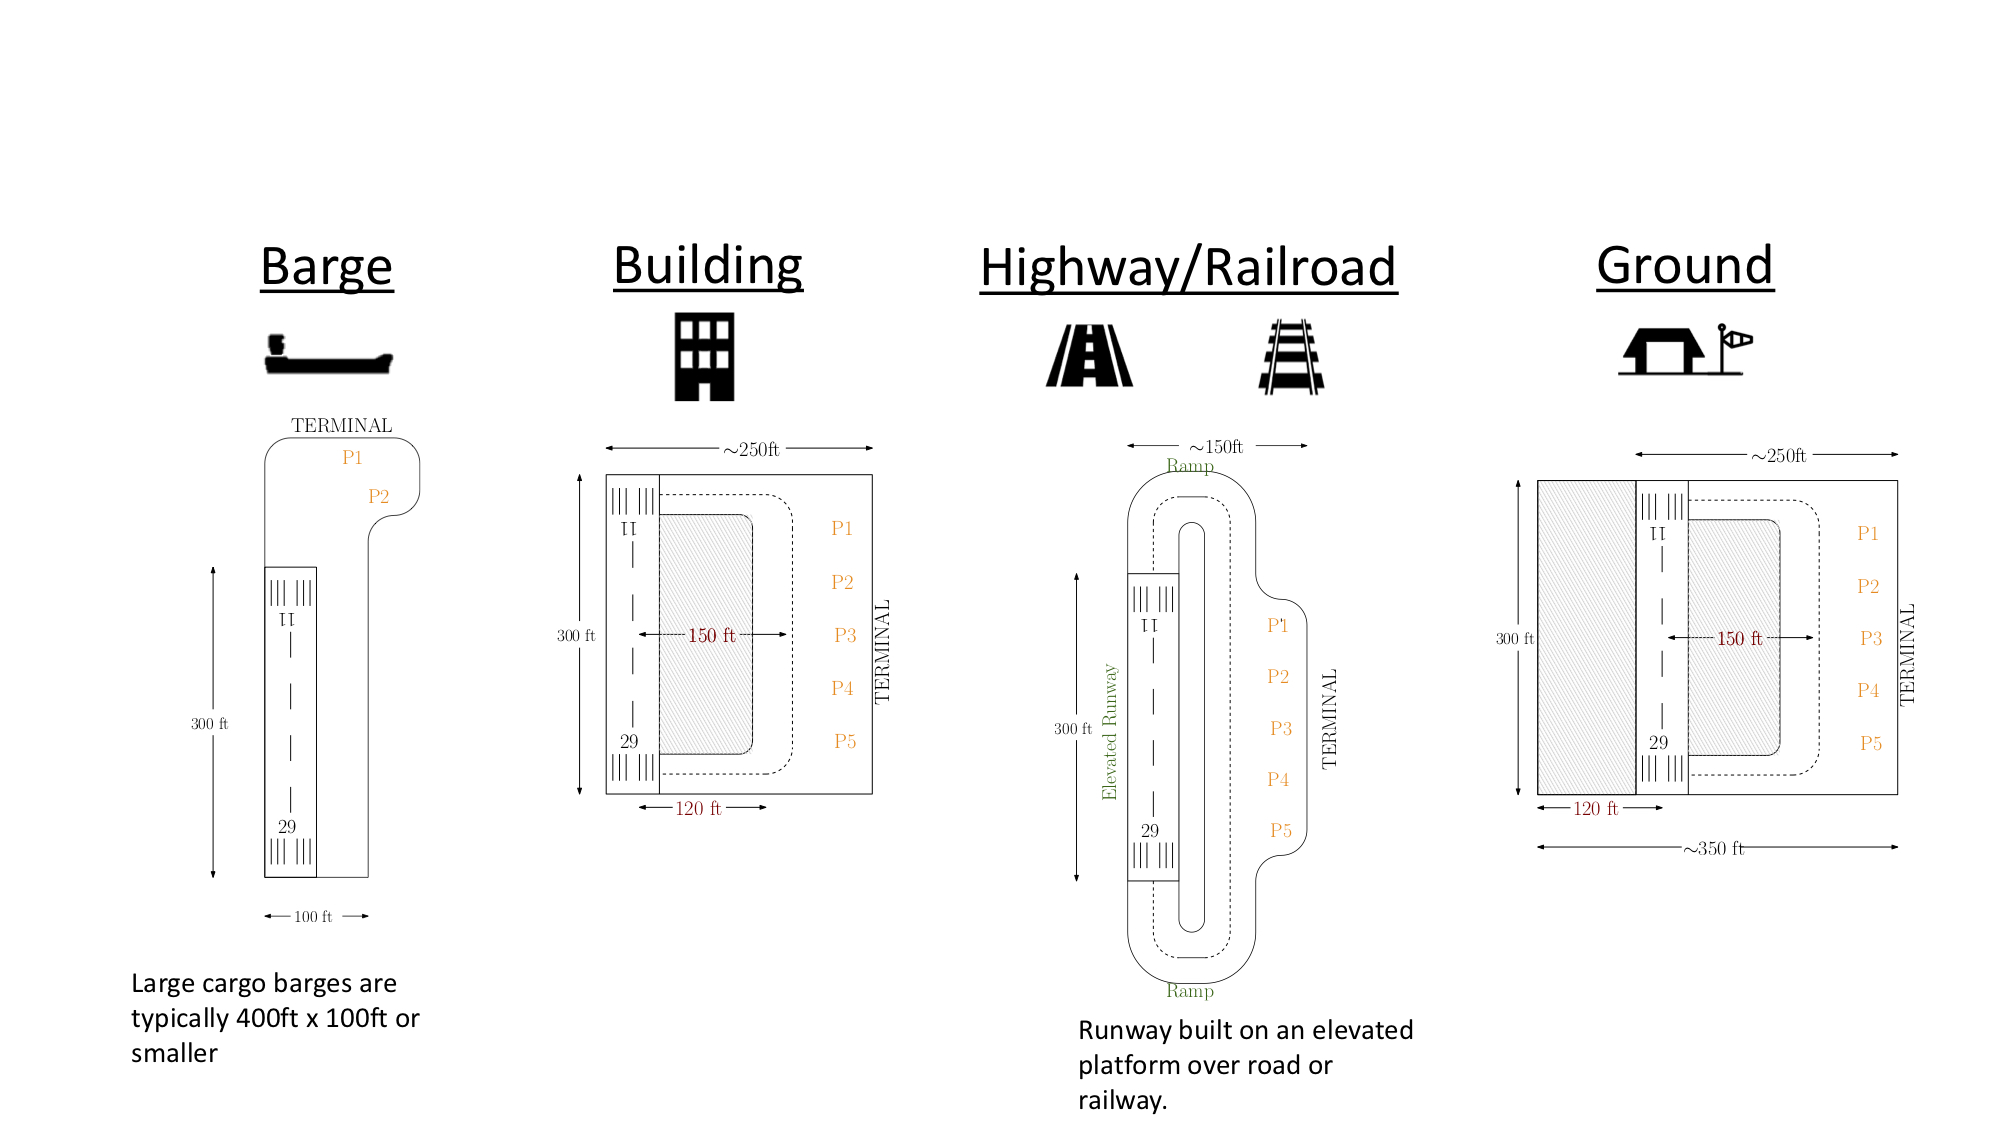
\includegraphics[width=1\textwidth]{STOLport_key.jpg}
\caption{Notional STOLport layouts for various locations}
\label{fig:stola_key}
\end{figure}
Future work will lay out more fully the design constraints of a notional STOLA, how the throughput is constrained by various systemic factors (vehicle separation, charging time/infrastructure, ground access, passenger loading times), and how that is reflected in the vehicle design. 

\section{Vehicle Feasibility}

A sizing study using Geometric Programming optimization was performed to understand how vehicle performance and design would be effected by short take offs and landings. 
This section describes the assumptions and equations used in the optimization model for vehicle size, cruise performance, and takeoff and landing distances.

Geometric programming was selected as a means of evaluating this trade space because of its speed and reliability.  
Geometric programming is a special type of convex, non-linear optimzation.\cite{gp}
Because it is convex, even GPs with thousands of variables can be solved quickly.\cite{gp}
Additionally, recent research has shown that GPs can be used to evaulate aircraft design trade spaces.\cite{burton_solar_2017}\cite{gpkit}


\subsection{Vehicle Model}

It is assumed that the aircraft is completely electric, replying on battery power for powered flight. 
The aircraft weight is comprised of the battery, payload, wing, motor, and structural weight,

\begin{equation}
    W_{\mathrm{MTO}} \geq W_{\mathrm{batt}} + W_{\mathrm{pay}} + W_{\mathrm{wing}} + W_{\mathrm{motor}} + W_{\mathrm{struct}}
\end{equation}

where the motor and structural weights are

\begin{align}
    W_{\mathrm{motor}} &\geq \frac{P_{\mathrm{shaft-max}}}{P_{\mathrm{spec}}} \\
    W_{\mathrm{struct}} &\geq W_{\mathrm{MTO}}f_{\mathrm{struct}}.
\end{align}

The battery weight is constrained by the range of the aircraft

\begin{equation}
    R \leq \frac{h_{\mathrm{batt}} W_{\mathrm{batt}} \eta_{\mathrm{elec}} V}{gP_{\mathrm{shaft}}}
\end{equation}

where the shaft power is 

\begin{equation}
    P_{\mathrm{shaft}} \geq \frac{TV}{\eta_{\mathrm{prop}}}
\end{equation}

The aircraft is assumed to be in steady level flight during cruise. 

The wing weight is composed of the skin, main spar and additional components

\begin{equation}
    W_{\mathrm{wing}} \geq W_{\mathrm{skin}} + W_{\mathrm{spar}} + W_{\mathrm{fadd}}
\end{equation}

The skin and structural elements are assumed to be carbon fiber.  
The wing spar configuration is a cap spar with unidirectional carbon fiber caps wrapped in a shear web as shown in Figure~\ref{f:capspar}.  

\begin{figure}[h!]
	\begin{center}
	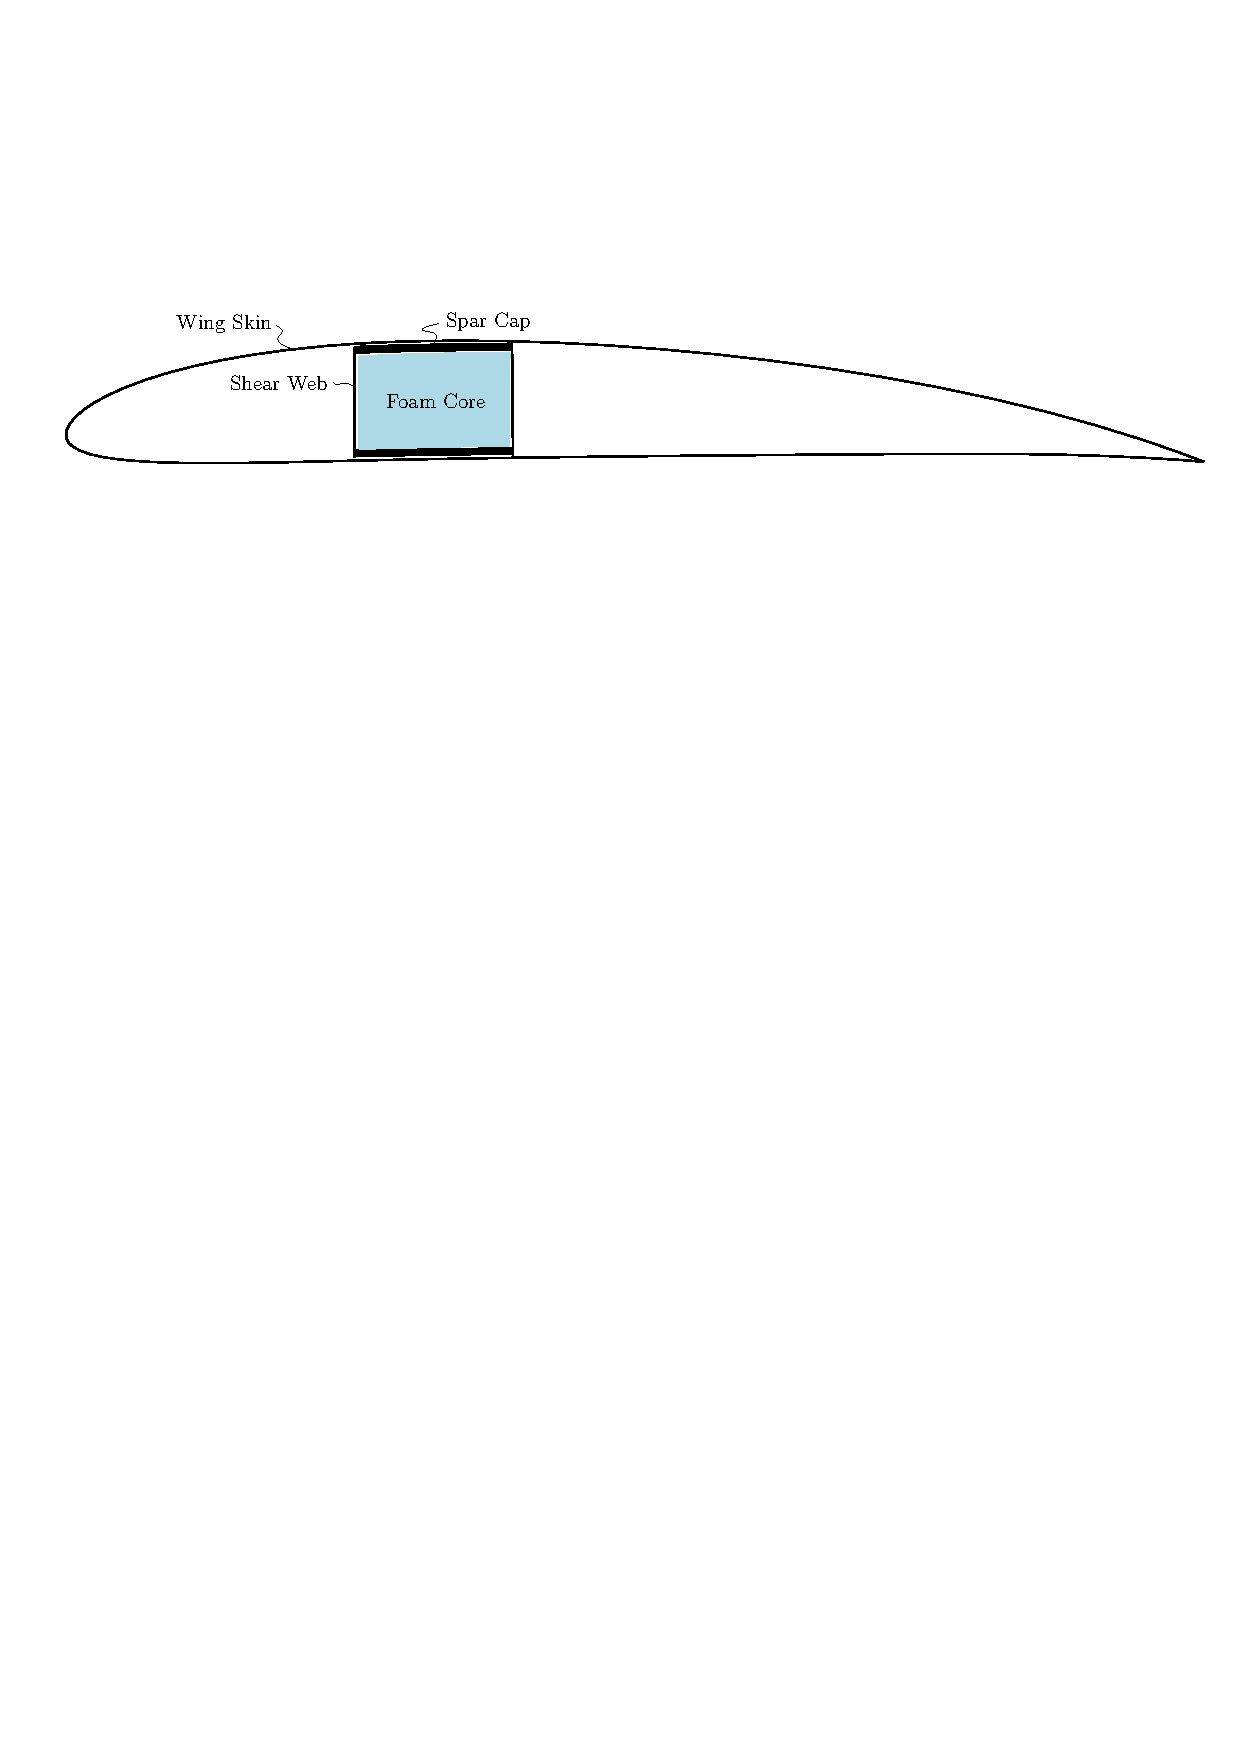
\includegraphics[width=0.9\textwidth]{capspar.pdf}
    \caption{\textbf{Cross sectional view of a cap spar.}}
	\label{f:capspar}
	\end{center}
\end{figure}

The spar dimensions are sized such that the material stresses are not exceeded under a 3.5 g-load,

\begin{equation}
    \sigma_{\mathrm{CFRP}} \geq \frac{\mathcal{M}_{\mathrm{root}}}{S_{y_{\mathrm{spar}}}}
\end{equation}

The root wing moment $\mathcal{M}_{\mathrm{root}}$, is calculated assuming a distributed load along the wing span that scales with the local chord.\cite{bending}
A constant tapered wing is assumed.  
This wing sizing model leverages the GP wing sizing model used by Burton and Hoburg.\cite{burton_solar_2017} 

A simple drag model is used for the aircraft, 

\begin{equation}
    C_D \geq CDA + c_{d_p} + \frac{C_L^2}{\pi e AR}.
\end{equation}

where the profile drag coefficient $c_{d_p}(C_L, Re)$, is calculated from a representative wing polar. 
The combined drag and wing loading models allow the aspect ratio to be optimized, trading structural integrity with aerodynamic performance. 

\subsection{Takeoff and Landing Models}

The takeoff model was adapted from Raymer's takeoff equations to fit a GP compatible form.  Using equations of motion the takeoff state can be expressed

\begin{equation}
    T - D - \mu(W_{\mathrm{MTO}} - L) = \frac{W_{\mathrm{MTO}}}{g} \frac{dV}{dt}.
\end{equation}

This can be simplified to 
\begin{align}
    \frac{dV}{dt} &= g \left( \frac{T}{W_{\mathrm{MTO}}} - \mu \right) - \frac{g}{W_{\mathrm{MTO}}} \left( \frac{1}{2} \rho S V^2 (C_{D_g} - \mu C_{L_g})\right) \\
    \label{e:todiff}
    \frac{dt}{dV} &= \frac{1}{A-BV^2}
\end{align}

The takeoff ground run distance can then be expressed by taking the integral of Equation~\ref{e:todiff} to achieve

\begin{equation}
    \label{e:to}
    S_{\mathrm{TO}} = \frac{1}{2B} \ln{\frac{A}{A-BV^2}} 
\end{equation}

The natural log function can be approximated to make Equation~\ref{e:to} GP-comptible by 

\begin{equation}
    \ln{\frac{A}{A-BV^2}} \approx \num{5.6e-4} A^{-6.04} (BV^2)^{6.04} + 1.0 A^{-0.001} (BV^2)^{0.001} + \num{7.5e-4} A^{-1.276} (BV^2)^{1.275}
\end{equation}

with an average log error of 0.06\%.  The terms $A$, and $B$, are constrained by

\begin{align}
    \frac{T}{W_{\mathrm{MTO}}} &\geq \frac{A}{g} + \mu \\
    B &\geq \frac{g}{W_{\mathrm{MTO}}} \frac{1}{2} \rho S C_{D_g}
\end{align}

where the $\mu C_{L_g}$ term is neglected as a conservative approximation for $B$ to preserve GP-compatibility. 

It is assumed that the primary constraint on landing is a comfortable deceleration for passengers.  
This constraint will drive the wing loading down. 

\begin{equation}
    S_{\mathrm{land}} \geq \frac{1}{2} \frac{V^2}{Ng} 
\end{equation}

where $N$ is the acceleration factor such that $N=1$ corresponds to a 1-g deceleration. 

For both the landing and takeoff constraints it is assumed that the velocity has a 20\% margin on the stall velocity,

\begin{equation}
    V = 1.2V_{\mathrm{stall}} = \sqrt{\frac{2W_{\mathrm{MTO}}}{\rho S C_{L_{\mathrm{max}}}}}.
\end{equation}

Another 40\% margin is placed on the ground roll distance to determine runway length

\begin{align}
    S_{\mathrm{runway}} &\geq 1.4S_{\mathrm{TO}} \\
    S_{\mathrm{runway}} &\geq 1.4S_{\mathrm{land}} 
\end{align}

\subsection{Vehicle Trade Studies}

Using the geometric programming model of a STOL aircraft perviously described, tradeoffs between runway length and vehicle performance were evaulated.  The models consists of a 105 free variables and was solved in 0.114 seconds with an objective function to minimize weight, $\min{(W_{\mathrm{MTO}})}$. Key parameters are defined in Table~\ref{t:params} and important solution variables are shown in Table~\ref{t:vars}.

\begin{multicols}{2}

\begin{table}[H]
    \centering
    \caption{Design Parameters}
    \label{t:params}
    \begin{tabular}{l c}
    \toprule
    \toprule
    Parameter                                   & Value \\ \hline
    $S_{\mathrm{runway}}$                       & 300 [ft] \\
    $W_{\mathrm{pay}}$                          & 800 [lbf] \\
    $\eta_{\mathrm{elec}}$                      & 0.9\\
    $h_{\mathrm{batt}}$                         & 210 [Whr/kg]\\
    $P_{\mathrm{spec}}$                         & 0.7136 [kW/N] \\
    $R$                                         & 100 [nmi] \\
    $C_{L_{\mathrm{max}}}$                      & 3.5 [kts] \\
    $\eta_{\mathrm{prop}}$                      & 0.8  \\
    \bottomrule
\end{tabular}
\end{table}

\begin{table}[H]
    \centering
    \caption{Design Parameters}
    \label{t:vars}
    \begin{tabular}{l c}
    \toprule
    \toprule
    Parameter                                   & Value \\ \hline
    $W_{\mathrm{MTO}}$                          & 1496 [lbf] \\
    $W_{\mathrm{batt}}$                         & 278 [lbf] \\
    $W_{\mathrm{wing}}$                         & 53 [lbf] \\
    $AR$                                        & 9 \\
    $b$                                         & 22.3 [ft] \\
    $V_{\mathrm{stall}}$                        & 48 [kts] \\
    $(W/S)$                                     & 27 [lbf/ft$^2$] \\
    \bottomrule
\end{tabular}
\end{table}

\end{multicols}

To understand how range and runway requirements affect vehicle weight, the GP model was solved 30 times in 3.46 seconds.  The results are shown in Figure~\ref{f:mtowrangew}, each point on the graph corresponding to a unique optimization solution or vehicle size.  
From this study it is observed that for runway lengths greater than about 350 ft, range is the constraining factor for vehicle weight.  
Conversly, while extemely short runways may be possible, it would come at the cost of vehicle range. 

\begin{figure}[h!]
	\begin{center}
	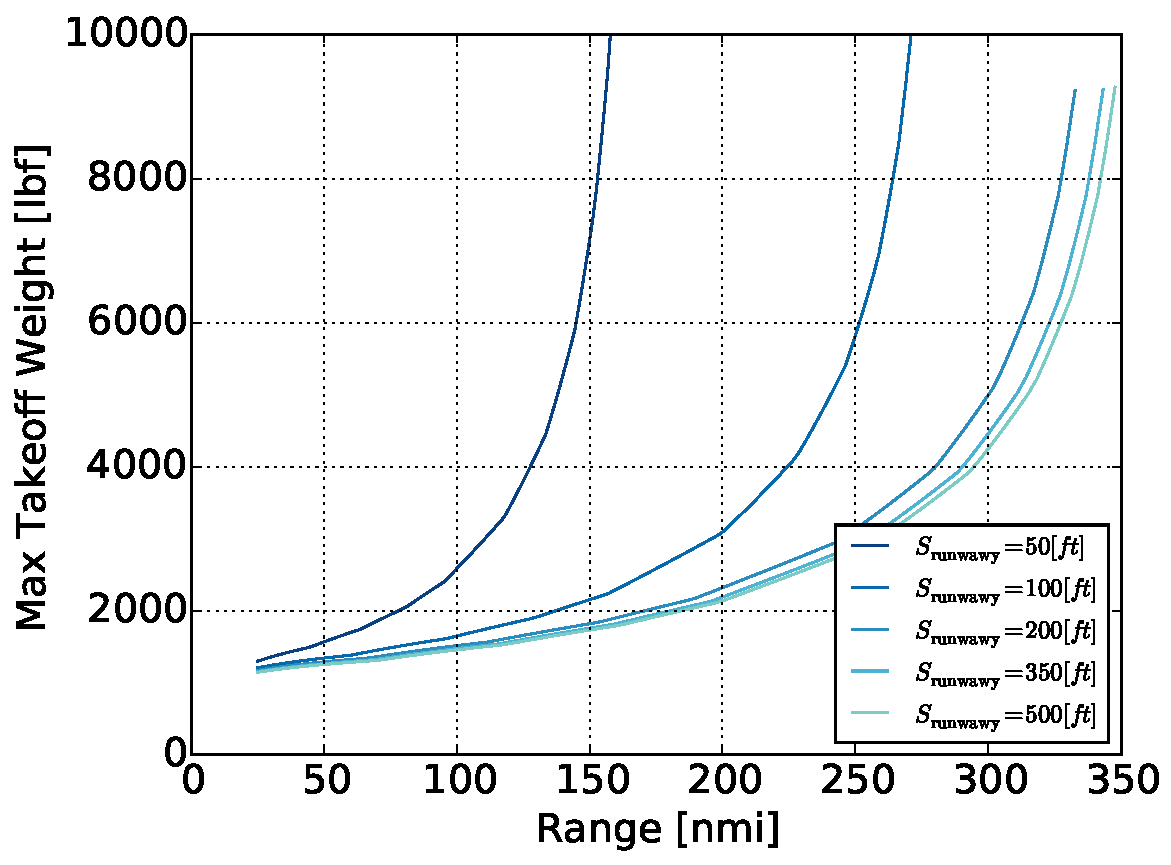
\includegraphics[width=0.6\textwidth]{mtowrangew.pdf}
    \caption{\textbf{Trade space of aircraft weight, range and runway length.}}
	\label{f:mtowrangew}
	\end{center}
\end{figure}

Another way to view this trade space is to understand how runway length and range trade for different max lift coefficients.  
Blow wings, highly cambered airfoils, or deflected wing surfaces can act to achieve higher max lift coefficients.  
Because the max lift coefficient for landing and takeoff may be different two separate studies were done, trading runway distance and vehicle range for different max lift coefficients, shown in Figure~\ref{f:rangetod}.  
Figure~\ref{f:rangetodclto} shows that higher lift coefficients on takeoff have little effect on the range of the aircraft.  
This is because the aircraft is constrained by the landing model and not the take off model.  
In Figure~\ref{f:rangetodclland}, the differenet lift coefficient lines converge around runway lengths of 150 ft.  
Therefore, for runway lengths greater than 150 ft vehicle range, not runway distance, becomes the driving requirement. 

\begin{figure}[h!]
 \begin{subfigmatrix}{2}% number of columns
     \subfigure[\label{f:rangetodclto}]{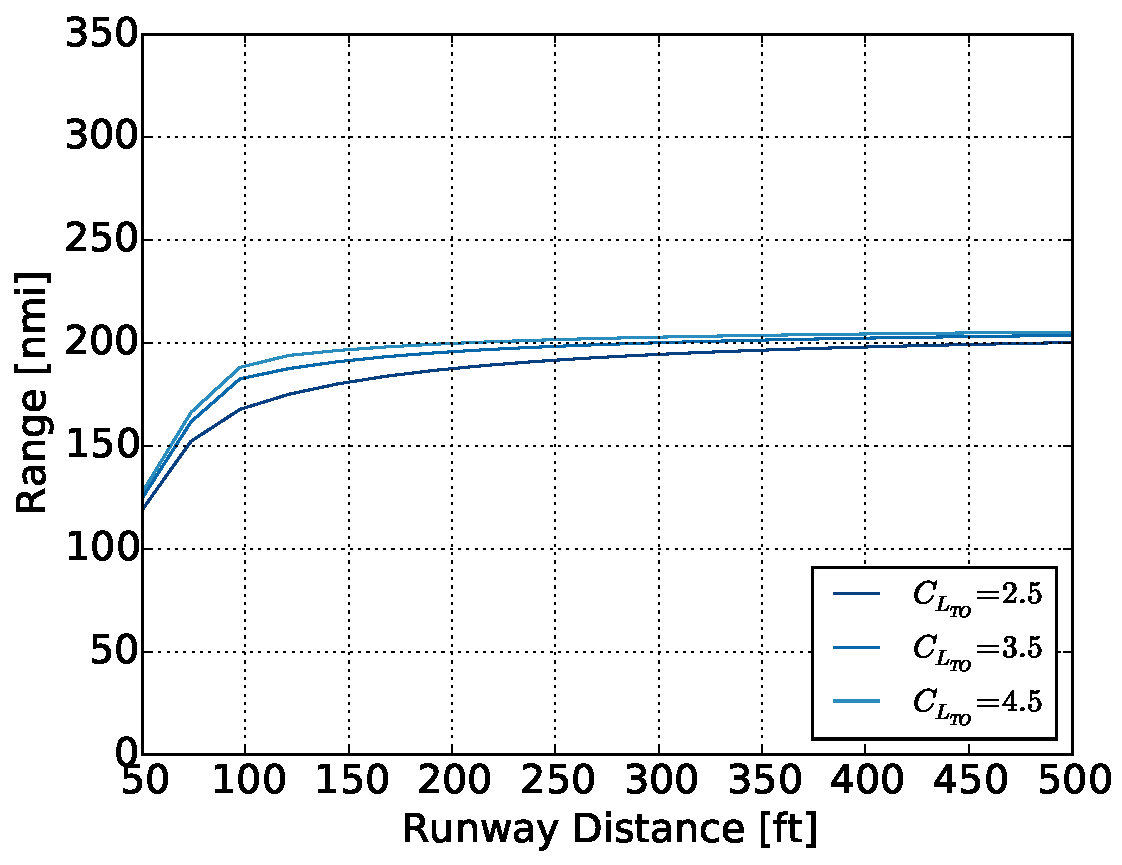
\includegraphics[]{rangetodclto.pdf}}
     \subfigure[\label{f:rangetodclland}]{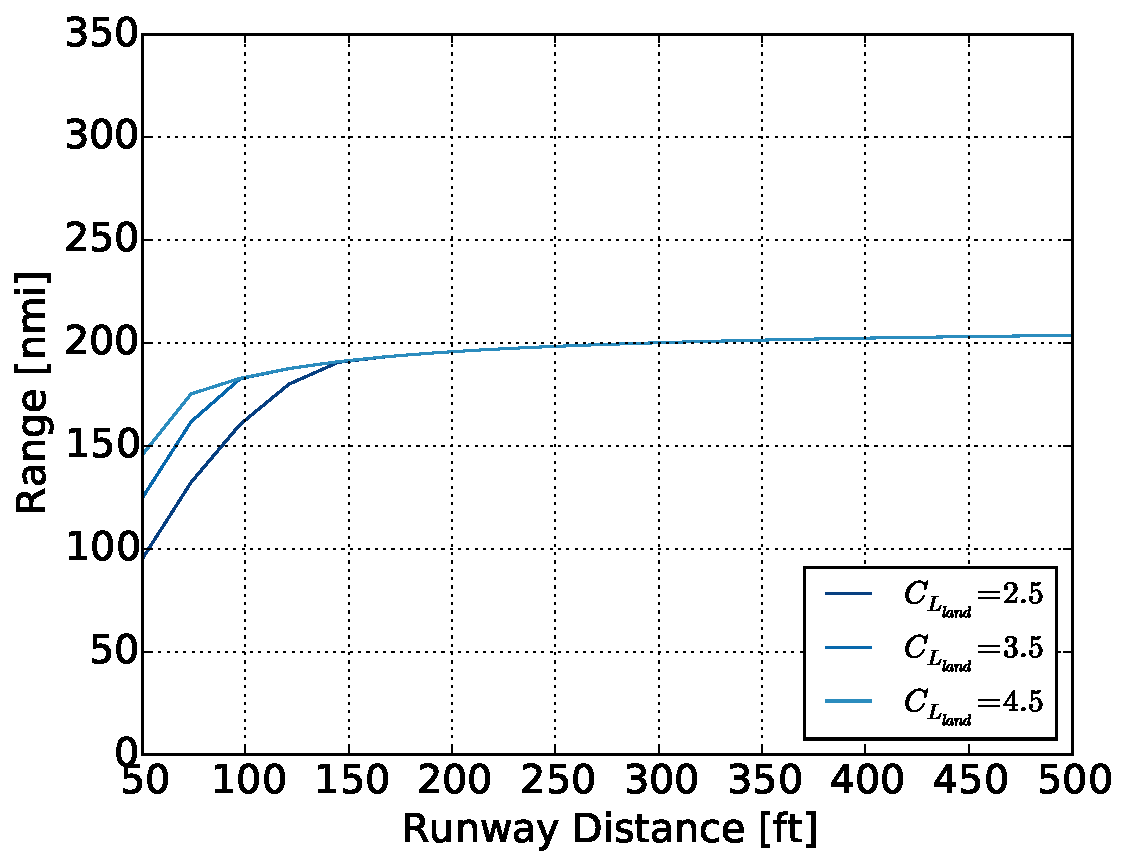
\includegraphics[]{rangetodclland.pdf}}
 \end{subfigmatrix}
 \caption{\textbf{Runway distance versus range for different maximum lift coefficients. }}
 \label{f:rangetod}
\end{figure}

These trade studies, done with simple models, show that there could likely be a realizable design of a short take off and landing vehicle that meets urban infrastructure requirements without a large penalty in performance.

\section{Market Analysis}

The first case study is the layout of an ESTOL UAM network in Boston, shown in Figure~\ref{fig:bos_network}.  This shows places where it may be feasible to locate a STOLA, normally focused on dual-use infrastructre.  These locations are chosen both so that they are near existing noise sources, away from dense residential areas, and connect to the existing high-throughput ground transportation networks.  
\begin{figure}[!htbp]
\centering
	\includegraphics[width=1\textwidth]{boston_layout.png}
\caption{Example layout of a STOL UAM network in Boston}
\label{fig:bos_network}
\end{figure}



\section{Conclusion}

\bibliography{biblibrary}
\bibliographystyle{aiaa}

\end{document}

